%!TEX root = ../../../memoria.tex
\section{Características actuales}

Como se explico en la \refSection{cap:arquitectura:section:generic_architecture_structure}, fue necesario desarrollar una arquitectura genérica para el desarrollo de aplicaciones en \meteorNAME con el fin de generar código de calidad. Acto seguido se comenzo con la implementación de las siguientes características:

\subsection{Cuestas de usuarios}
 
%Meteor Accounts
%Meteor Accounts is a complete user account system that you can drop into your application. With one line of code, you can have login, logout, account creation, email validation, password recovery, and login with OAuth providers like Facebook or Twitter.
Existe un sistema completo de cuentas de usuarios el cual permite hacer \loginCPT(\refFigura{figure:account:sign_in_ui}), \logoutCPT(\refFigura{figure:account:log_out}), creación de cuentas (\refFigura{figure:account:create_account}), y recuperacion de contraseña\refFigura{figure:account:reset_password}). Aunque en estricto rigor, la recuperación de contraseña momentaneamente corresponde a una contraseña aleatoria generada por la aplicación y enviada al correo.


\begin{figure}[H]
	\centering
	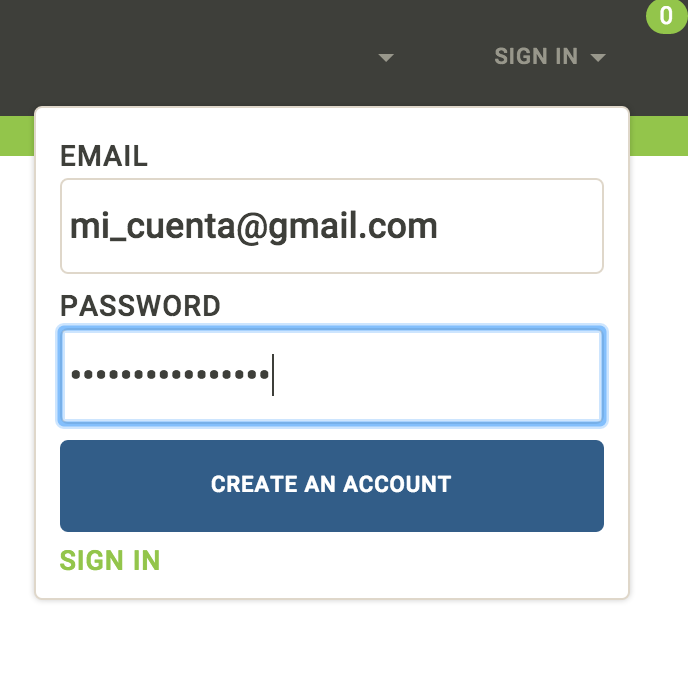
\includegraphics[width=0.3\textwidth]{figuras/accounts/create_account.png}

	\caption{Creación de una cuenta.}
	\label{figure:account:create_account}
\end{figure}

\begin{figure}[H]
	\centering
	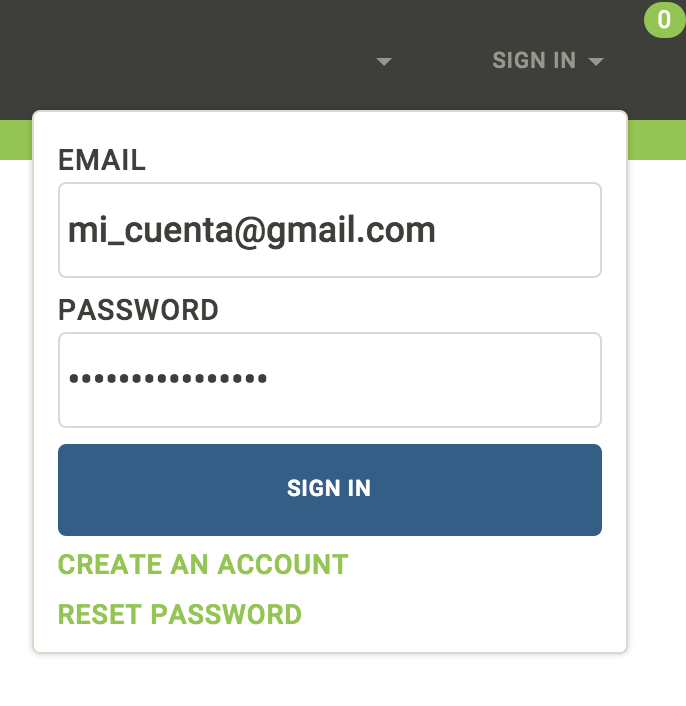
\includegraphics[width=0.3\textwidth]{figuras/accounts/sign_in_ui.png}

	\caption{Autenticarse en la aplicación.}
	\label{figure:account:sign_in_ui}
\end{figure}


\begin{figure}[H]
	\centering
	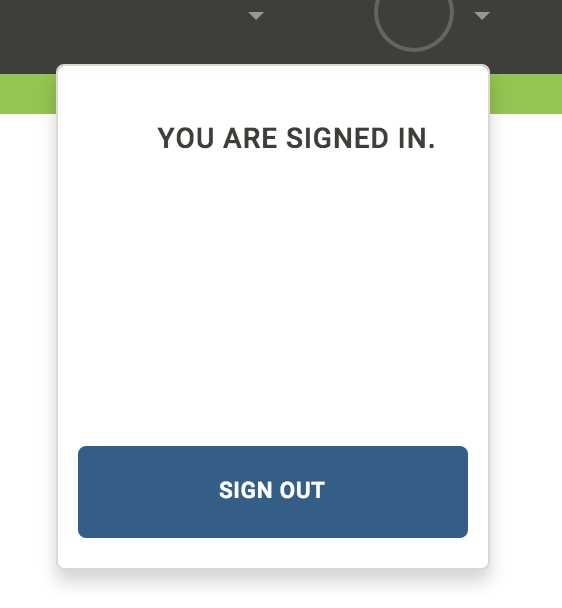
\includegraphics[width=0.3\textwidth]{figuras/accounts/log_out.png}

	\caption{Desvincular la cuenta de la aplicación.}
	\label{figure:account:log_out}
\end{figure}

\begin{figure}[H]
	\centering
	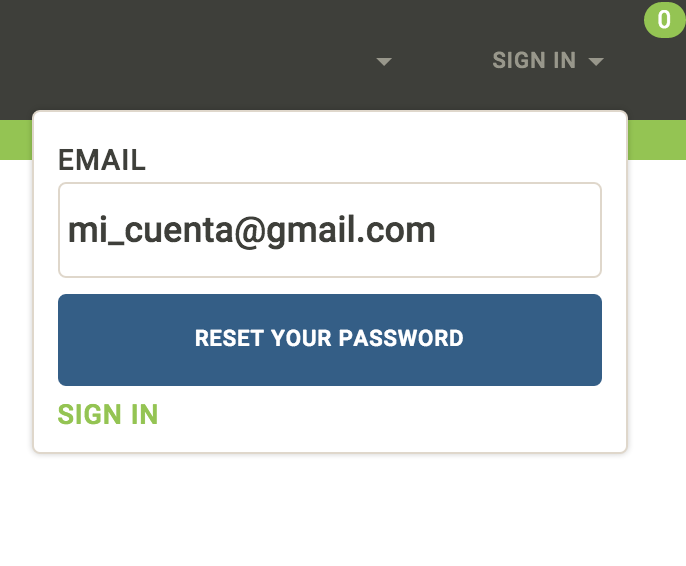
\includegraphics[width=0.3\textwidth]{figuras/accounts/reset_password.png}

	\caption{Reset contraseña.}
	\label{figure:account:reset_password}
\end{figure}

demás el sistema permite hacer \loginCPT a traves de un servicio de autenticación \thirdParty tales como \facebook, \googleNAME, \twitterNAME, \gitHubNAME, entre otros utilizando los \packagesAS de \meteorNAME \accountFacebook, \accountGoogle, \accountTwitter y \accountGithub respectivamente. En la \refFigura{figure:account:log_in_plus_facebook} se observa la existencia de un servicio \thirdParty para la autenticación en la aplicación.


\begin{figure}[H]
	\centering
	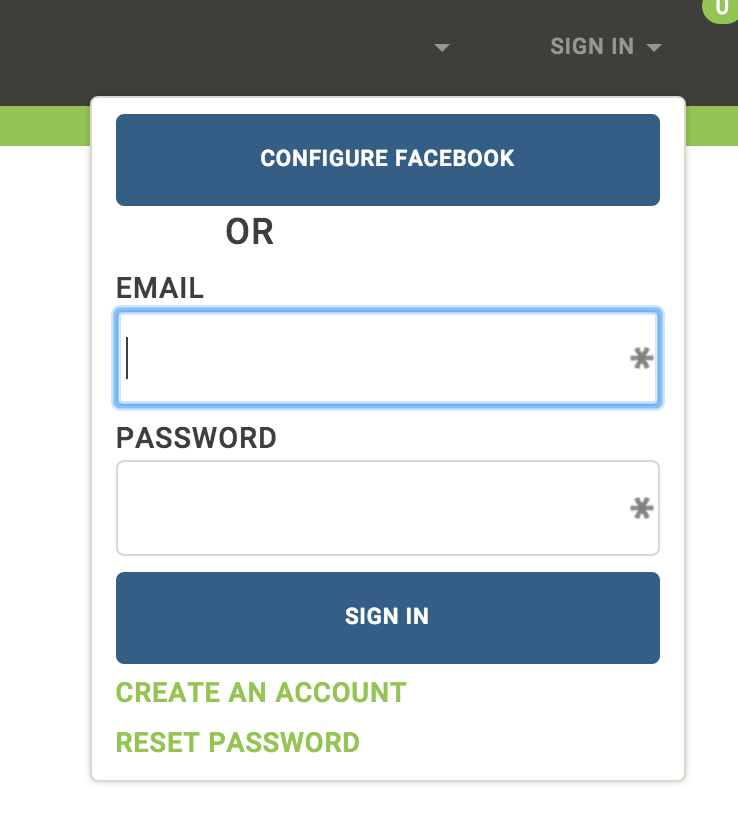
\includegraphics[width=0.3\textwidth]{figuras/accounts/log_in_plus_facebook.png}

	\caption{Autenticarse utilizando un servicio \thirdParty.}
	\label{figure:account:log_in_plus_facebook}
\end{figure}

Es importante agregar que el sistema automáticamente agrega en la interfaz la opción de autenticarse utilizando el servicio \thirdParty simplemente agregando el \packagesAS de \meteorNAME; y por consiguiente este desaparecerá si el \packagesAS es removido. En la \refFigura{figure:account:log_in_all_package} se aprecian varios servicios \thirdParty para la autenticación de la aplicación.

\begin{figure}[H]
	\centering
	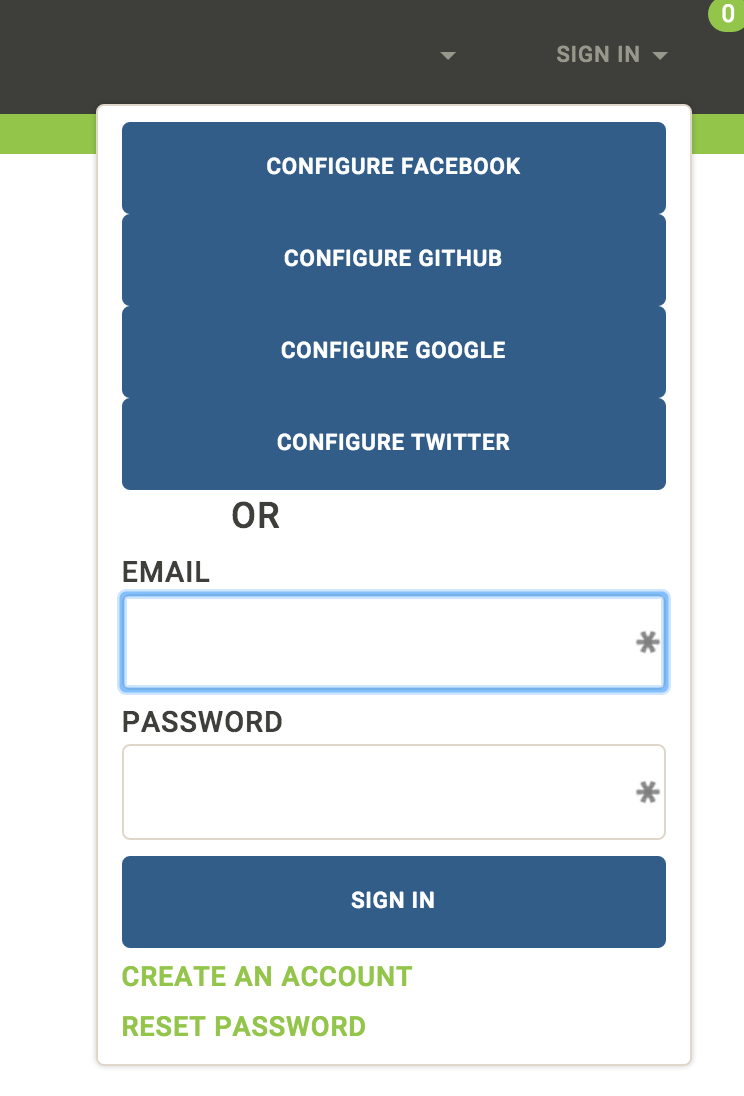
\includegraphics[width=0.3\textwidth]{figuras/accounts/log_in_all_package.png}

	\caption{Autenticarse utilizando uno de varios servios \thirdParty.}
	\label{figure:account:log_in_all_package}
\end{figure}


%you can provide your own UI for these features or you can even use a premade boilerplate UI to get up and running quickly.

%eteor Accounts is a modular system, and anyone can write a package that provides a new login method. Some, but not all of these packages are officially maintained by the Meteor Project. For example, accounts-password has a complete password-based login system, including password recovery. Packages such as accounts-google, accounts-facebook, and accounts-twitter provide the ability to log in with common third-party authentication services.

%The account database is stored in a users database collection that is automatically created on the server. Currently this can only be stored in MongoDB, but other databases will likely be supported in the future, depending on demand. The schema of this database is shown in the main Meteor docs.

%Passwords are safely encoded with bcrypt according to industry best practices.

\subsection{Localización}

Ingles no solo ostenta el primer lugar como el idioma más utilizado. \rankingCPT que considera además del porcentage de población, la distribución geográfica. Si no que además es el idioma más utilizado en los \websitesINT alcanzando la cifra de 59,4\%. Seguido tímidamente por Rusia con un 5.9\% \cite{online_world_wide_languages}. Mirando estas cifras se podría concluir que la inclusión de múltiples idiomas en un \siteINT \ecommerceCOM	no reprensentaría ingresos importantes.
El potencial económico \online es de \$45 trillones, de acuerdo a un estudio realizado por \commonSenseAdvisoryNAME \cite{online_world_global_oportunity_multi_languages}.  Sin una solida estrategia de localización que considere \websitesINT \ecommerceCOM con multi-idiomas, será  un desafio tener al alcanze de la mano ese \revenueCOM. De hecho, el mismo estudio vislumbró que si solo se tiene una versión en ingles del  \siteINT, se estará limitado solo a una tercera parte del total.

%Grow revenue with website localization
%The economic potential of online communication is $45 trillion, according to a recent study by Common Sense Advisory. How exciting! The sky is the limit for your global business.
%Or is it?
%Without a solid localization strategy that incorporates an e-commerce website in multiple languages, it will be a challenge to get within arm’s reach of this revenue. In fact, the same study found that if you have just an English version of your website, you’re limited to only one third of the pot.

¿Cuántos serán los idiomas necesarios para permanecer competitivo en el mundo \online. Los investigadores dicen que un mínimo de 14. Las marcar mundiales que aspiran a un 95\% de las billeteras \online necesitan de 20 idiomas. Si bien es cierto, no es siempre posible mantener contenido \online en 20 idiomas, es dificil negar los beneficios de la localización para regiones específicas al rededor del mundo \cite{online_world_global_oportunity_multi_languages}. Estan son las razones de por que se considera muy importante la localización en el \frameworkPC y de por que se aborda esta caracteristica desde los inicios.

Actualmente la aplicación cuenta con un sistema robusto para la localización, permitiendo nuevos idiomas simplemente agregando un archivo \jsonNAME. En la \refFigura{figure:features:languages_available}
%How many languages does it take for global businesses to stay competitive online? The research says a minimum of 14. Global brands wanting to appeal to 95 percent of the world’s online wallet need 20 languages. While it isn’t always feasible for a business to translate online content into 20 languages, it’s hard to deny the benefits of website localization for targeted regions around the world.
%Many businesses recognize this and plan to add even more languages to their localization strategy in the future. One example is European-based clothing seller ASOS. They launched a website for the Chinese and Russian markets in 2013 to expand their global footprint. They already had a presence in the United Kingdom, United States, France, Germany and Australia. They saw international sales overall increase by 39 percent with their past website localization initiatives—so they knew that additional language sites would help grow revenue.
%If you’re ready to get a bigger piece of the global e-commerce pie, like ASOS, consider upping the number of languages on your website. Check out the article, Global e-commerce: Are these 5 items in your localization shopping cart?, for tips on how to approach e-commerce website localization.


\begin{figure}[H]
	\centering
	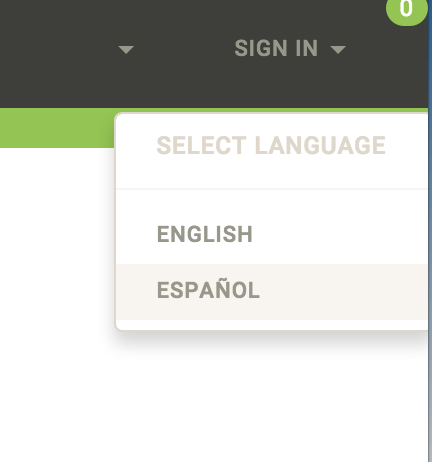
\includegraphics[width=0.3\textwidth]{figuras/accounts/languages_available.png}

	\caption{Selección de idioma para el \websitesINT.}
	\label{figure:features:languages_available}
\end{figure}


\subsection{Descripción de un producto}

La aplicación permite consultar la descripción de un producto. Dicha interfaz puede observarse en la \refFigura{igure:bootstrap:theme_cyborg}. Se puede aprenciar alguans de las carecteristicas de las que ya dispone cada producto.

\begin{itemize}
	\item
		Un título del producto.
	\item
		Un subtítulo para dar un resumen.
	\item
		Un espacio para la foto del producto.
	\item
		Un lugar para la descripción del producto.
	\item
		Un precio ó intervalo de precios.
\end{itemize}

Si bien es cierto, esta interfaz no tiene aún todas las caracteristicas usualmente visibles en los \websitesINT \ecommerceCOM típicos, son un paso intermedío hacia esa finalidad.

 \subsection{Edición de un producto}

Actualmente puede asociarce un creador a un producto (usando \fixturesPC) y por lo tanto solo aquel tendra acceso a editar, eliminar, y proximamente ocultar el producto.

Para editar los campos, simplemente es necesario seleccionar la componente con el \mouse y hacer un \click. La componente cambiara su aspecto para dar \feedback al usuario de que esta seleccionada la componente y que puede realizar ediciones sobre el campo. En la \refFigura{figure:features:interfaz_edicion_producto}, \refFigura{figure:features:interfaz_edicion_editando_description} y \refFigura{figure:features:interfaz_edicion_editando_subtitulo} es posible apreciar la componenete que se ha seleccionado para editar.

\begin{figure}[H]
	\centering
	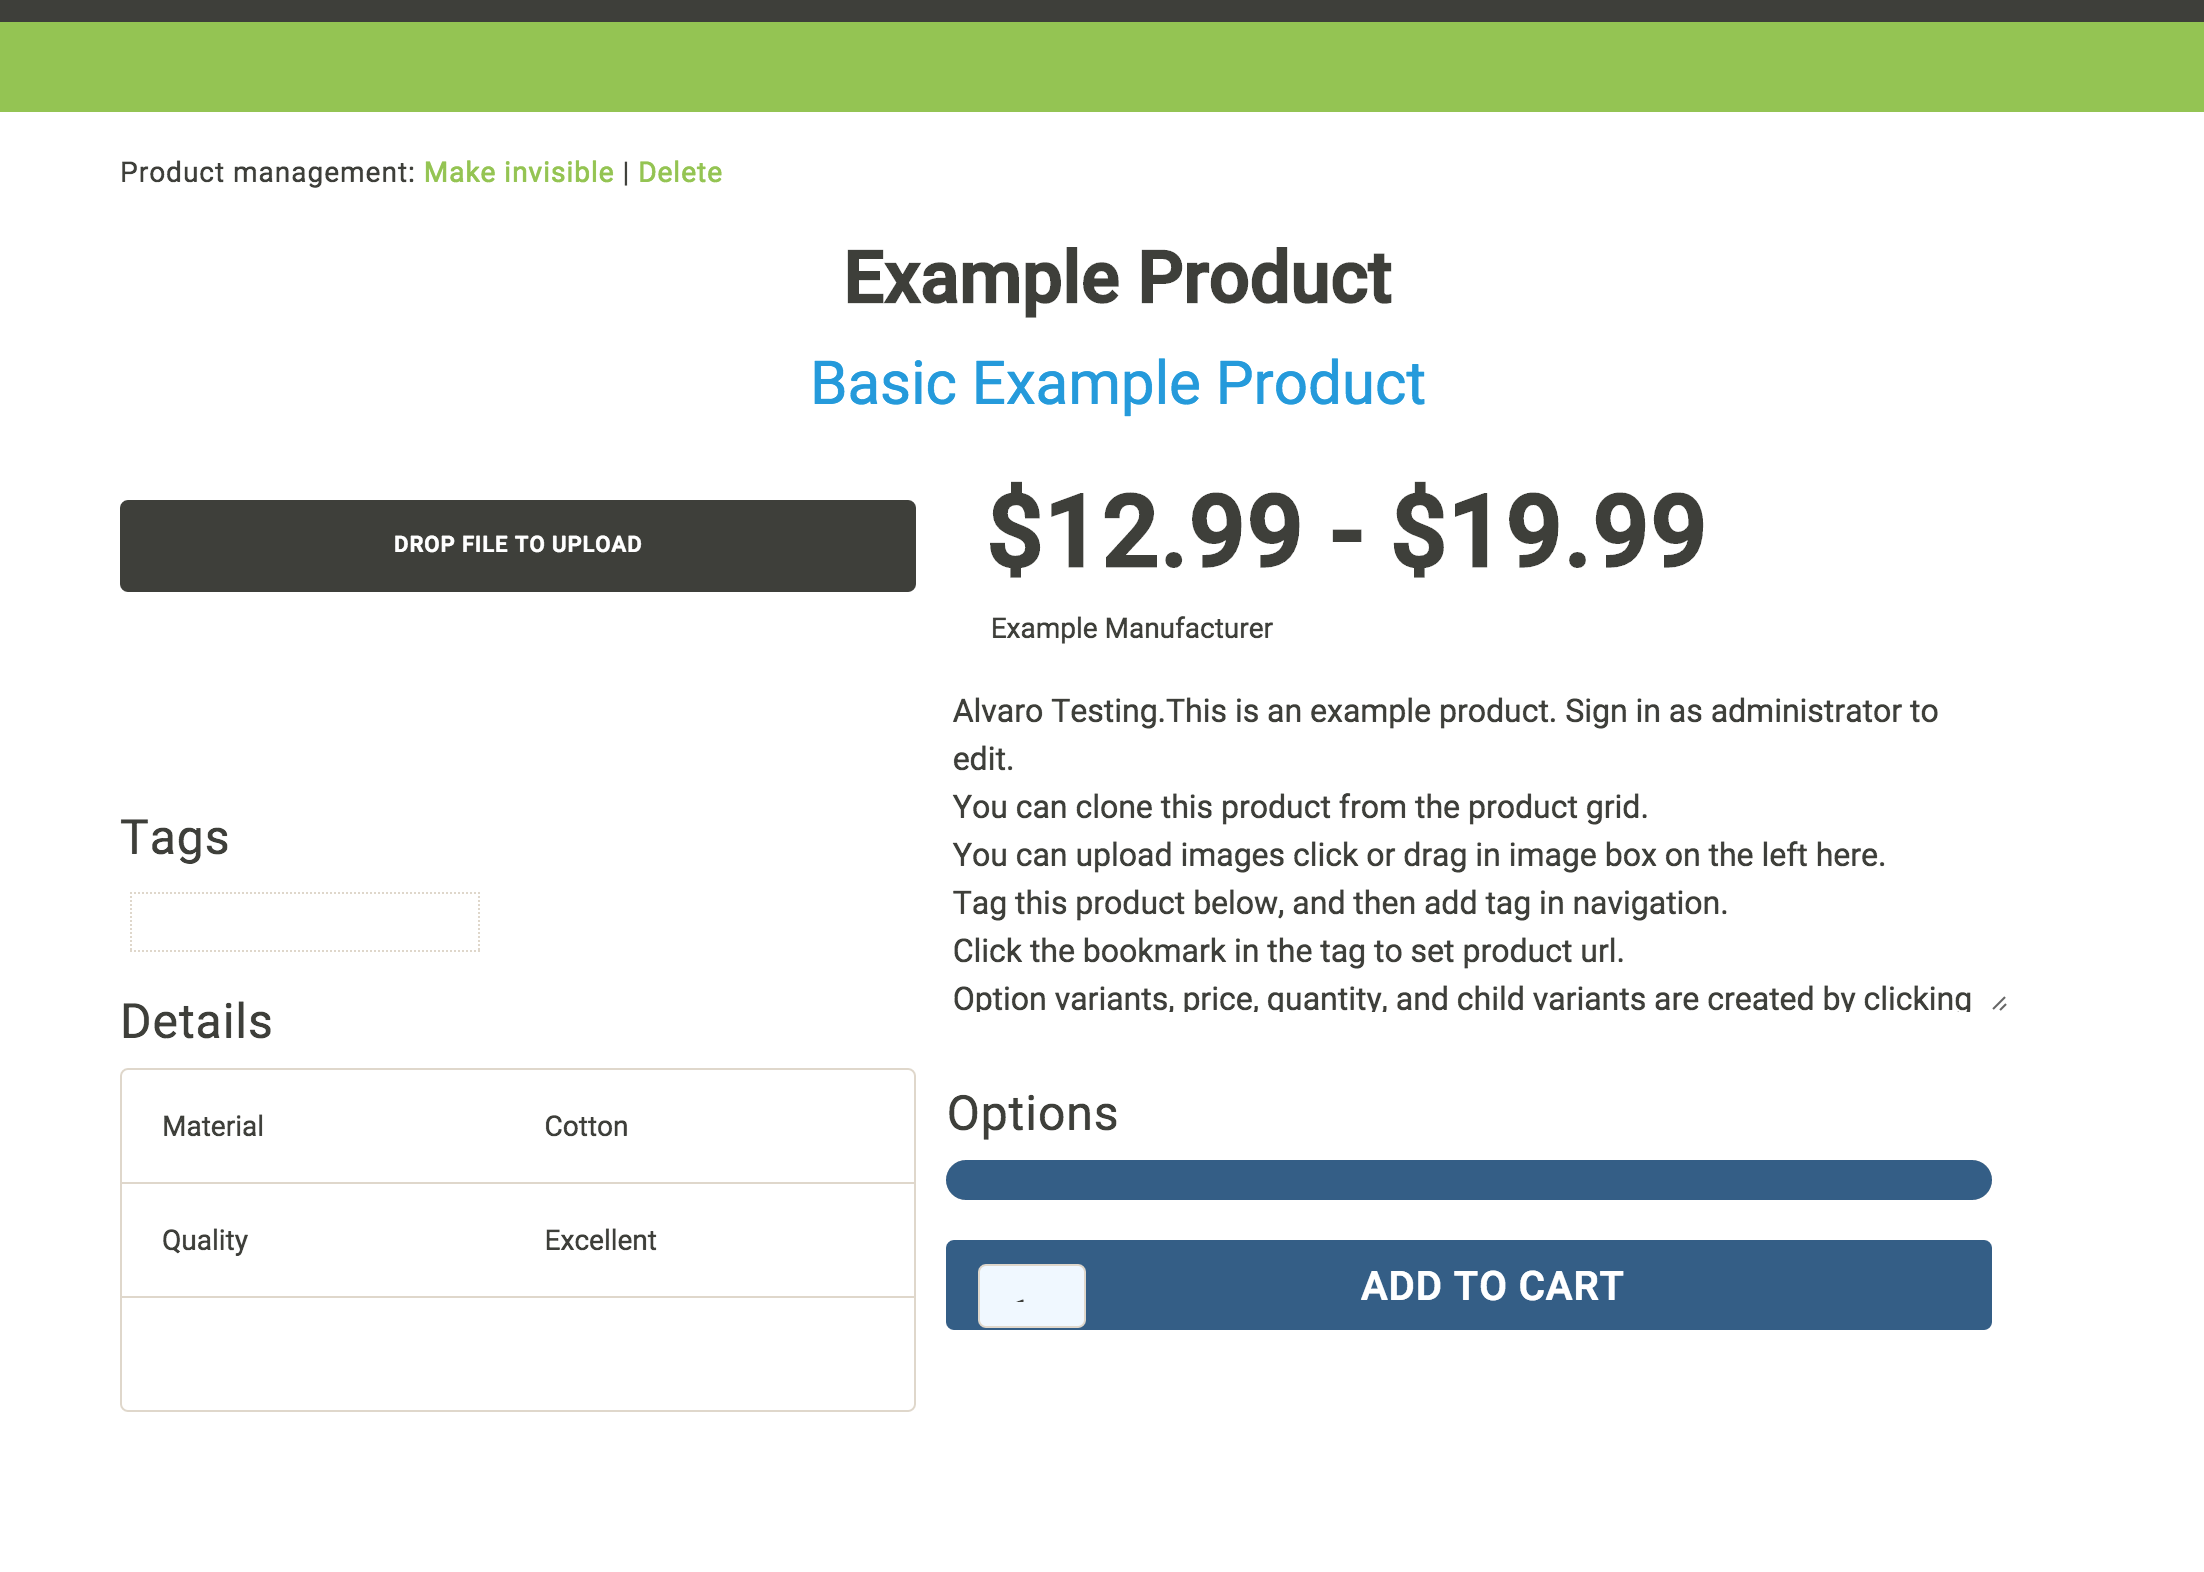
\includegraphics[width=0.3\textwidth]{figuras/productos/interfaz_edicion_producto.png}

	\caption{Interfaz de la edición de un producto.}
	\label{figure:features:interfaz_edicion_producto}
\end{figure}

\begin{figure}[H]
	\centering
	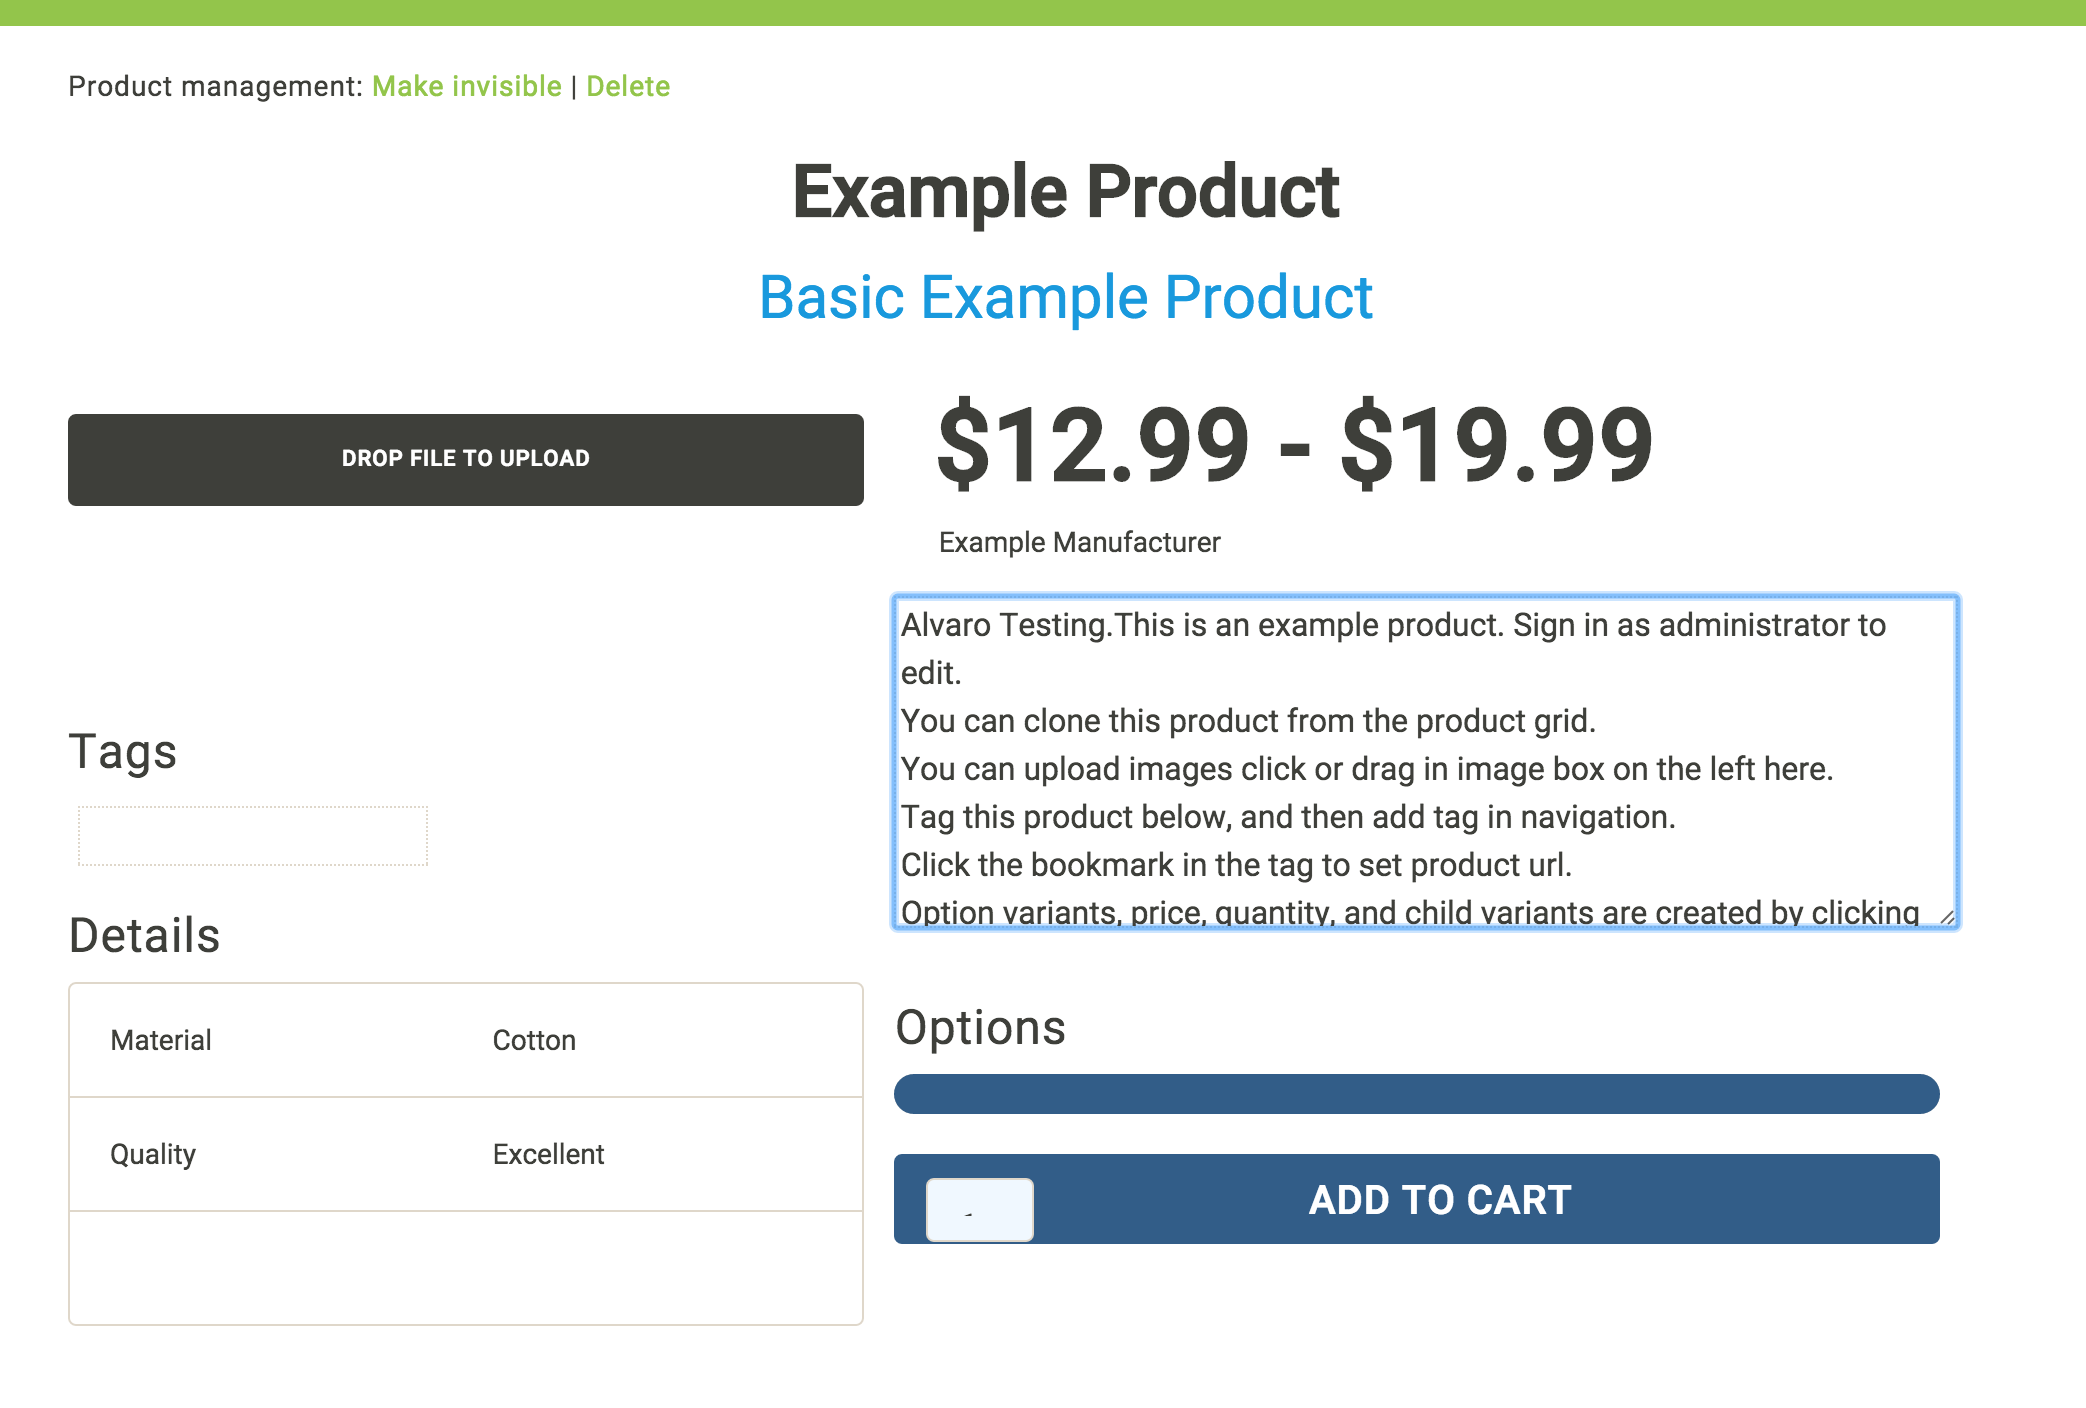
\includegraphics[width=0.3\textwidth]{figuras/productos/interfaz_edicion_editando_description.png}

	\caption{Campo descripción seleccionado para edición.}
	\label{figure:features:interfaz_edicion_editando_description}
\end{figure}


\begin{figure}[H]
	\centering
	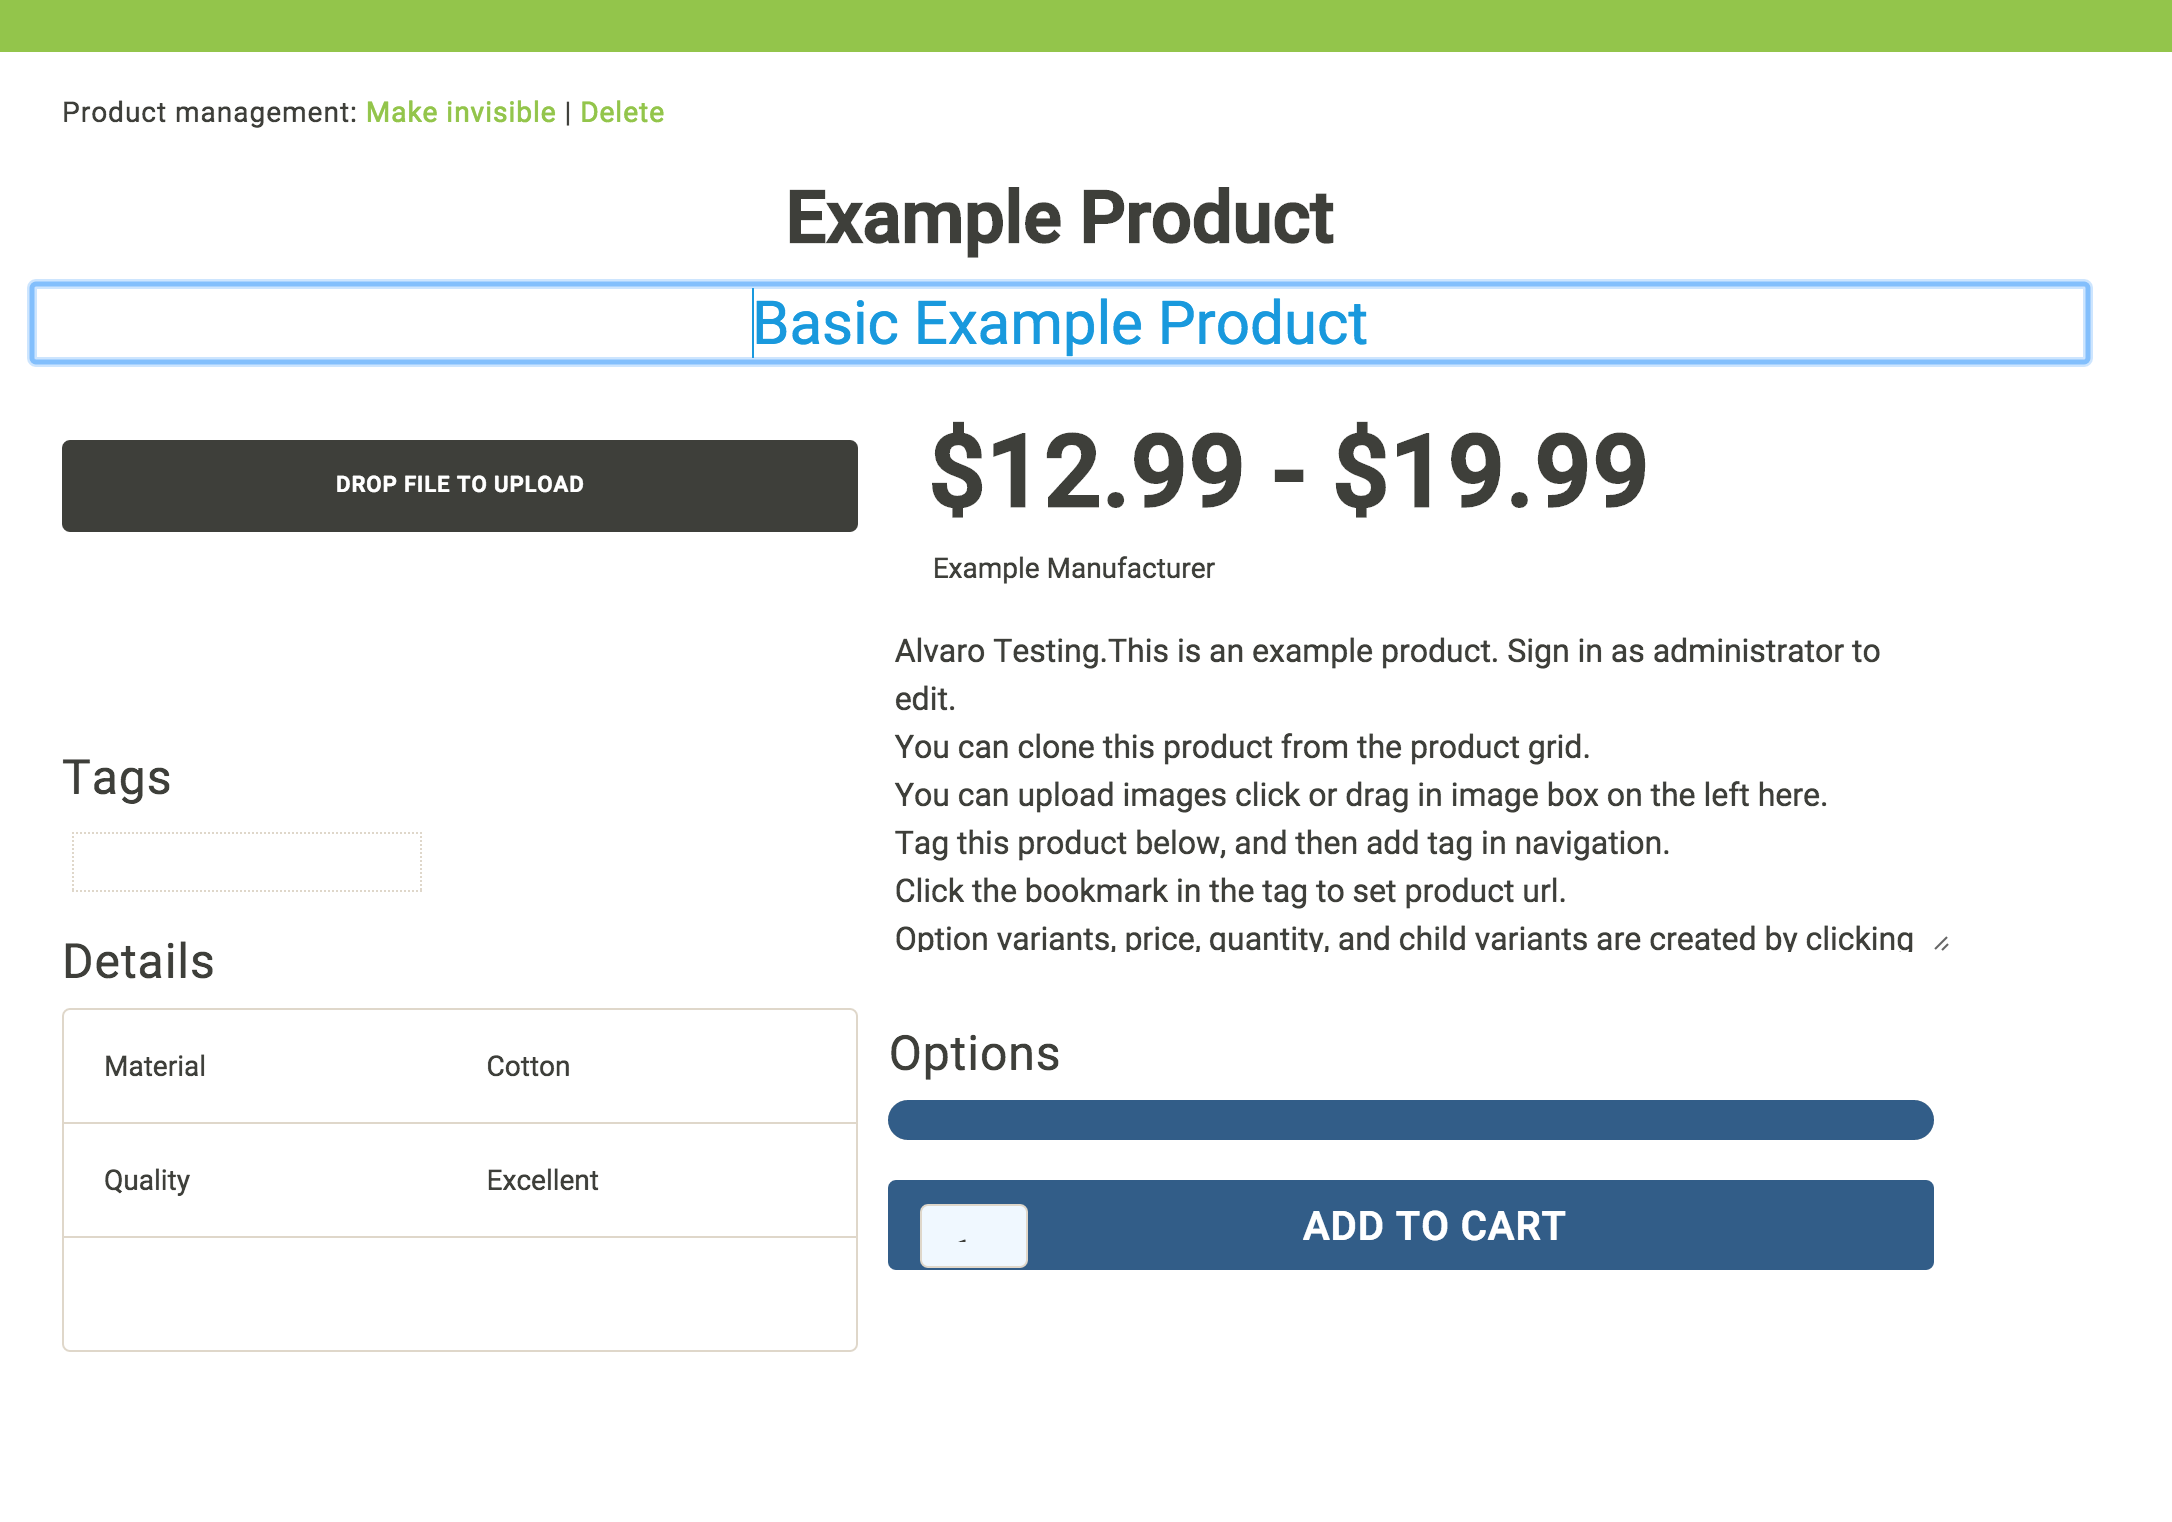
\includegraphics[width=0.3\textwidth]{figuras/productos/interfaz_edicion_editando_subtitulo.png}

	\caption{Campo subtítulo seleccionado para edición.}
	\label{figure:features:interfaz_edicion_editando_subtitulo}
\end{figure}

